
%+++++++++++++++++++++++++++++++++++++++++++++++++++++++++++++++
% SUMMARY    : Lecture 19 
%            : Optimizers
%            : University of Southern Maine 
%            : @james.quinlan
%            : Abdullahi Abdullahi - Lecture 19, 04/28/2025
%+++++++++++++++++++++++++++++++++++++++++++++++++++++++++++++++
\section*{Objectives}
\begin{itemize}
    \item Neural Network Architecture
    \item How to Train a Network
    \item Feedforward Networks
    \item Backpropagation Algorithm
    \item Cost Function Minimization
    \item Chain Rule Application
\end{itemize}

\section{Neural Network Architecture}

\subsection{How to Train a Network}
\begin{itemize}
    \item Forward Feed
    \item Calculate cost (loss/error)
    \item Backpropagation
    \item GOTO 1 (repeat) (Until cost $\approx 0$)
\end{itemize}

\subsection{Feedforward Neural Networks}
A  neural network consists of multiple layers of neurons where connections between neurons do not form cycles. Information moves in only one direction - forward - from the input nodes, through the hidden nodes, to the output nodes.

We organize our network into $L$ layers:
\begin{itemize}
    \item Input layer (indexed as $l=1$)
    \item Hidden layers (indexed as $l=2, \ldots, L-1$)
    \item Output layer (indexed as $l=L$)
\end{itemize}

Each layer contains a set of neurons (nodes). As shown in our notes:
\begin{itemize}
    \item Now we have a total of $L$ layers
    \item Each neuron is connected to neurons in adjacent layers
\end{itemize}

\begin{figure}[h]
\centering
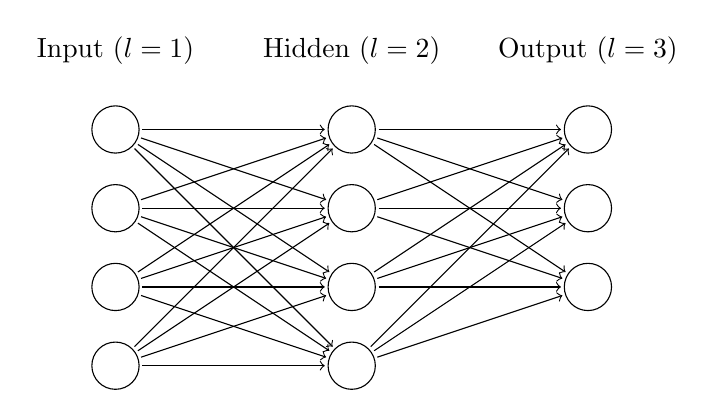
\begin{tikzpicture}[
    node distance=1.5cm,
    neuron/.style={circle, draw, minimum size=0.6cm},
    arrow/.style={->, shorten >=1pt, shorten <=1pt}
]

% Input layer
\node[neuron] (i1) at (0,2) {};
\node[neuron] (i2) at (0,1) {};
\node[neuron] (i3) at (0,0) {};
\node[neuron] (i4) at (0,-1) {};
\node at (0, 3) {Input ($l=1$)};

% Hidden layer
\node[neuron] (h1) at (3,2) {};
\node[neuron] (h2) at (3,1) {};
\node[neuron] (h3) at (3,0) {};
\node[neuron] (h4) at (3,-1) {};
\node at (3, 3) {Hidden ($l=2$)};

% Output layer
\node[neuron] (o1) at (6,2) {};
\node[neuron] (o2) at (6,1) {};
\node[neuron] (o3) at (6,0) {};
\node at (6, 3) {Output ($l=3$)};

% Connect input to hidden
\foreach \i in {1,...,4}
    \foreach \j in {1,...,4}
        \draw[arrow] (i\i) -- (h\j);

% Connect hidden to output
\foreach \i in {1,...,4}
    \foreach \j in {1,...,3}
        \draw[arrow] (h\i) -- (o\j);

\end{tikzpicture}
\caption{A feedforward neural network with 3 layers ($L=3$)}
\end{figure}

\subsection{Indices and Notation}
As seen in our notes, we use superscript $(l)$ to denote the layer number:
\begin{itemize}
    \item $x^{(l)}$ indicates indices
    \item $i, j, k$ are used as indices
\end{itemize}

For a network with $n$ input neurons, $m$ hidden neurons, and $k$ output neurons:
\begin{itemize}
    \item Each neuron in a layer is connected to every neuron in the next layer
    \item All of these connections have weights associated with them
\end{itemize}

\subsection{Matrix Representation}
Every neuron in the hidden layer is connected to neurons from the previous layer. We can represent the connections using matrix notation:

For a neuron $i$ in layer $l$, we compute its activation $a_i^{(l)}$ as:
\begin{equation}
a_i^{(l)} = \sigma\left(\sum_{j=1}^{n^{(l-1)}} w_{ji}^{(l)} a_j^{(l-1)} + b_i^{(l)}\right)
\end{equation}

Where:
\begin{itemize}
    \item $w_{ji}^{(l)}$ is the weight connecting the $j$-th neuron in layer $l-1$ to the $i$-th neuron in layer $l$
    \item $b_i^{(l)}$ is the bias for the $i$-th neuron in layer $l$
    \item $\sigma$ is the activation function
    \item $n^{(l-1)}$ is the number of neurons in layer $l-1$
\end{itemize}

In matrix form, we can write this as:
\begin{equation}
\mathbf{a}^{(l)} = \sigma(\mathbf{W}^{(l)} \mathbf{a}^{(l-1)} + \mathbf{b}^{(l)})
\end{equation}

Where:
\begin{equation}
\mathbf{a}^{(l)} = 
\begin{bmatrix}
a_1^{(l)} \\
a_2^{(l)} \\
\vdots \\
a_{n^{(l)}}^{(l)}
\end{bmatrix},
\mathbf{W}^{(l)} = 
\begin{bmatrix}
w_{11}^{(l)} & w_{12}^{(l)} & \ldots & w_{1n^{(l-1)}}^{(l)} \\
w_{21}^{(l)} & w_{22}^{(l)} & \ldots & w_{2n^{(l-1)}}^{(l)} \\
\vdots & \vdots & \ddots & \vdots \\
w_{n^{(l)}1}^{(l)} & w_{n^{(l)}2}^{(l)} & \ldots & w_{n^{(l)}n^{(l-1)}}^{(l)}
\end{bmatrix},
\mathbf{b}^{(l)} = 
\begin{bmatrix}
b_1^{(l)} \\
b_2^{(l)} \\
\vdots \\
b_{n^{(l)}}^{(l)}
\end{bmatrix}
\end{equation}

\section{Cost Function Minimization}

\subsection{Objective Function}
Our objective is to minimize the cost function $C$. As noted in our class:
\begin{equation}
\text{obj: minimize } C
\end{equation}

The cost function is typically defined as:
\begin{equation}
C = \frac{1}{2}\sum_j (a_j^{(L)} - y_j)^2
\end{equation}

Where:
\begin{itemize}
    \item $a_j^{(L)}$ is the output of the $j$-th neuron in the output layer
    \item $y_j$ is the corresponding target value (ground truth vector)
\end{itemize}

\subsection{Backpropagation Algorithm}
To minimize the cost function, we need to compute its gradient with respect to the weights and biases. The backpropagation algorithm allows us to do this efficiently.

\subsubsection{Forward Pass}
The forward pass computes the activations of all neurons in the network:
\begin{equation}
z^{(l)} = w^{(l)} \cdot a^{(l-1)} + b^{(l)}
\end{equation}
\begin{equation}
a^{(l)} = \sigma(z^{(l)})
\end{equation}

Where $\sigma$ is the activation function.

\subsubsection{Backward Pass}
In the backward pass, we compute the error terms for each neuron and propagate them backward through the network.

The error term for an output neuron $j$ is defined as:
\begin{equation}
\delta_j^{(L)} = \frac{\partial C}{\partial z_j^{(L)}} = \text{sensitivity}
\end{equation}

As noted in our calculations:
\begin{equation}
\delta_j^{(L)} = \frac{\partial C}{\partial z_j^{(L)}} = (a_j^{(L)} - y_j) \cdot \sigma'(z_j^{(L)})
\end{equation}

For a neuron in an earlier layer, we have:
\begin{equation}
\delta_j^{(l)} = \sum_k \delta_k^{(l+1)} w_{jk}^{(l+1)} \cdot \sigma'(z_j^{(l)})
\end{equation}

\subsection{Chain Rule Application}
The core of backpropagation is the application of the chain rule from calculus. As our notes indicate, we apply the chain rule to compute:
\begin{equation}
\frac{\partial C}{\partial w_{ij}^{(l)}} = \frac{\partial C}{\partial z_i^{(l)}} \cdot \frac{\partial z_i^{(l)}}{\partial w_{ij}^{(l)}} = \delta_i^{(l)} \cdot a_j^{(l-1)}
\end{equation}

Similarly, for the bias:
\begin{equation}
\frac{\partial C}{\partial b_i^{(l)}} = \frac{\partial C}{\partial z_i^{(l)}} \cdot \frac{\partial z_i^{(l)}}{\partial b_i^{(l)}} = \delta_i^{(l)}
\end{equation}

\subsection{Weight Update}
Once we have computed the gradients, we update the weights and biases:
\begin{equation}
w_{ij}^{(l)} = w_{ij}^{(l)} - \alpha \frac{\partial C}{\partial w_{ij}^{(l)}}
\end{equation}
\begin{equation}
b_i^{(l)} = b_i^{(l)} - \alpha \frac{\partial C}{\partial b_i^{(l)}}
\end{equation}

Where $\alpha$ is the learning rate.

\section{Summary}
To summarize what we've covered:
\begin{itemize}
    \item Neural networks consist of layers of interconnected neurons
    \item Each connection has an associated weight
    \item The forward pass computes the output of the network
    \item The cost function measures the error between the network’s output and the desired output
    \item Backpropagation uses the chain rule to compute the gradients of the cost function efficiently
    \item Gradient descent updates the weights and biases to minimize the cost function
\end{itemize}
